\subsection{Alumno}

  \paragraph{}Se procede a crear el usuario alumno, en este caso, el mencionado
  en el capítulo \ref{enunciado}, \textit{Enunciado}. Para ello, se realizará la
  creación de un alumno, tal y como se describió en el capítulo \ref{addAlumno},
  \textit{Añadir alumno}.

  \paragraph{}Una vez que aparezca el formulario de creación, se debe introducir
  el nombre del alumno y sus datos personales en el formulario, con lo que
  la pantalla quedaría tal y como refleja la figura \ref{ejemploAddAlumno}.

  \begin{figure}[!ht]
    \begin{center}
      \fbox{
      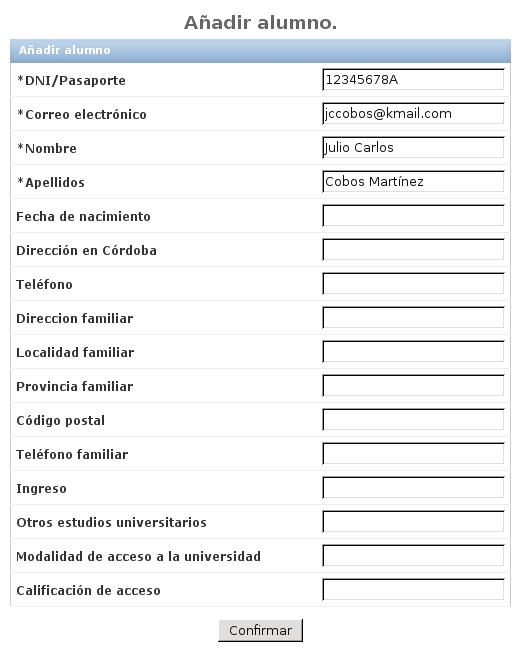
\includegraphics[scale=0.55]{5.Ejemplos_Practicos/5.3.IntroduccionDatos/5.3.8.Alumno/add_alumno.png}
      }
      \caption{Creación de \textit{Alumno} de ejemplo.}
      \label{ejemploAddAlumno}
    \end{center}
  \end{figure}

  \paragraph{}Una vez rellenado el formulario, se pulsará el botón
  \textit{Confirmar}, el cual se puede ver en la figura
  \ref{capturaBotonConfirmar}. Si el formulario rellenado es válido, y no tiene
  errores, se creará el nuevo elemento en el sistema. En caso de contener
  información no válida, un mensaje de error aparecerá indicando los campos
  del formulario que no han pasado la validación, los cuales habrá que modificar
  para introducir correctamente el elemento en el sistema.
